% Distributed under the Apache license, Version v2.0
% Copyright 2017 Felipe Estrada-Solano <festradasolano at gmail>
% Based on Keith A. Gillow's OCIAM Thesis lyx files
% ==============
% DOCUMENT CLASS
% ==============
%\documentclass[11pt,draft]{thesis_proposal-dtm_unicauca} % draft version
\documentclass[11pt,twoside]{thesis_proposal-dtm_unicauca} % submission version
% ==============
% LaTeX PACKAGES
% ==============
% -----
% Color
\usepackage{color}
% -----
% Fonts
\usepackage{lmodern}
\usepackage{helvet}
\renewcommand{\familydefault}{\sfdefault}
\usepackage[T1]{fontenc}
% -----------
% Other fonts
\usepackage{listings}
\usepackage{verbatim}
% -------
% Margins
\usepackage[letterpaper]{geometry}
\geometry{verbose,tmargin=3cm,bmargin=2.5cm,lmargin=3cm,rmargin=2.5cm,headheight=3cm,headsep=1cm}
% -----------
% Hyphenation
\usepackage[american]{babel}
% -------------
% Alignment
\usepackage{array}
% -------------
% External PDFs
\usepackage{pdfpages}
% ----
% Math
\usepackage{amsmath}
% -------
% Symbols
\usepackage{amssymb}
% --------
% Graphics
\usepackage{graphicx}
\graphicspath{{figures/}} % path(s)
%\DeclareGraphicsExtensions{.eps} % extension(s)
% ------------
% Bibliography
\usepackage[numbers]{natbib}
% ------------
% Period label separation instead of colon
\usepackage[labelsep=period]{caption}
% ----------------
% Hyper-references
\usepackage[unicode=true, bookmarks=true,bookmarksnumbered=true,bookmarksopen=false, breaklinks=true, pdfborder={0 0 0},backref=page,colorlinks=true]{hyperref}
% ----------------
% Table formatting
\usepackage{array}
\usepackage{multirow}
% ===============
% LaTeX UTILITIES
% ===============
% ----------------
% Hyper-references
\hypersetup{pdftitle={Links Utilization Prediction in SDN Based on Data Mining}, pdfauthor={Edwin Ferney Castillo Quintero}, colorlinks=true, citecolor=blue, linkcolor=black, urlcolor=green}
% ----------------
% Grayscale colors
% ---------------------------------------------------------------
% Pages with more than 80% of floats become pure float-only pages
\renewcommand{\floatpagefraction}{.8}%
% -----------------------
% Extra height for tables
\renewcommand{\arraystretch}{1.6}
% ==================
% DOCUMENT UTILITIES
% ==================
% -------------
% Unicauca logo
\def\logo{{
\includegraphics[scale=0.45]{logo_unicauca.pdf}}}
% ----------------------------
% Arguments for the cover page
\title{Intelligent Probing for SDN Monitoring}
\author{Edwin Ferney Castillo Quintero}
\degree{Master}
\program{Telematics Engineering}
\advisor{Oscar Mauricio Caicedo Rendon}
\advisordegree{Ph.D.}
\coadvisor{}
\coadvisordegree{}
\lineresearch{Advanced Services of Telecommunications}

\usepackage{datetime}
\newdateformat{monthyeardate}{%
  \monthname[\THEMONTH] \THEYEAR}
  
\submitmonth{\monthyeardate\today}
%\submityear{2017}
% If no co-advisor, do not comment, just define argument as empty
%\coadvisor{}
%\coadvisordegree{}
\coadvisor{}
\coadvisordegree{}
% -----------
% Hyphenation
%\catcode`\_=12
%\lccode`\_`\_
\hyphenation{}
% ========
% DOCUMENT
% ========
\begin{document}
% -----------------------------------------------
% Build the cover page (generated from arguments)
\pagenumbering{gobble}
\maketitle
% -----------
% Roman pages
\begin{romanpages}
% -----------------
% Table of contents
\pdfbookmark{\contentsname}{toc}
\renewcommand{\contentsname}{\LARGE\centerline{Contents}}
\tableofcontents{}
% ---------------
% List of figures
%\renewcommand{\listfigurename}{\LARGE\centerline{List of Figures}}-- comentado
%\listoffigures-- comentado
% --------------
% List of tables
%\renewcommand{\listtablename}{\LARGE\centerline{List of Tables}} -- comentado
%\listoftables -- comentado
% ---------------
% End roman pages
\end{romanpages}
\pagenumbering{arabic}
% ------------------------------
% Paragraph spacing for document
\setlength{\parskip}{1em}
% Paragraph spacing for sections in documents
\titlespacing\section{0pt}{12pt plus 4pt minus 2pt}{0pt plus 4pt minus 2pt}
% -----------------
% Problem Statement
\section{Problem Statement}
\label{sec:problem_statement}

%The exponential growth of IP traffic makes traditional networks very difficult to manage \cite{Jararweh_2015:sdn_iot}. This difficulty lies in the fact that administrators must deal with complex communication protocols (vendor-specific), network policy diffuse deployment and limited routing scalability \cite{Sterbenz_2013:taxonomy_n, anderson_da_silva_2015:resilience_sdn_survey, Klein_2013:of_omnet}. Even more, the network devices are vertically integrated: control plane and data plane embedded in the same hardware. Software-Defined-Networking (SDN) is a paradigm that promises to solve such difficulties, redefining the network architecture by separating between the control plane and the data plane, centralizing control logic and introducing the ability to program network \cite{kreutz_2015:sdn_comprehensive_survey, nunes_2014:surve_sdn_ppf}.

SDN provides a flexible architecture fast and easy configuration of network devices. In addition, it implements fine-grained network management based on the decoupling of the data and control planes \cite{herrera_2016:nfv_survey}. However, this separation is not enough to guarantee that the network will not degrade with the increment of traffic. In this sense, another important approach to optimize a network and improve network robustness is Traffic Engineering (TE) \cite{ian_2014:a_road_map_sdn}.

TE deals with measurement and management of network traffic aiming to improve the utilization of network resources and the associated Quality of Service (QoS). TE, in SDN, focuses on four approaches \cite{ian_2014:a_road_map_sdn, z_shu_2016:TE_SDN_measure_manage}: (\textit{i}) Flow Management that seeks to find both the solution to prevent network overload and the trade-off between latency and load balancing, (\textit{ii}) Fault Tolerance intends to ensure the immediate recovery of the network when a failure occurs in any node, (\textit{iii}) Topology Update aims to update the network policies in real time and ensure their application in each flow; and (\textit{iv}) Analysis/Characterization of traffic that is related to mechanisms for network monitoring, debugging, fault detection, and data collection.

An essential requirement for TE is to provide accurate and reliable traffic monitoring (e.g., Flow Management needs granular real-time monitoring information to compute the most efficient routing decisions). Traffic monitoring is fundamental to observe and quantify what is happening in the network, and it is closely related to Traffic Management mechanisms \cite{tangari_2017:decentralized_monitoring, machado_2014:towards_SLA_Policy}. For example, policy rules can be triggered by conditions monitored in the network (e.g., link congestion or bottleneck). Network traffic monitoring techniques can be classified into two categories \cite{mohan2011:active_passive,Ningning_2003:probing_techniques}: passive monitoring and active probing (also called active monitoring). Passive monitoring tools use the trace history of existing data transmission to analyze network health ``capture-and-analyze". Active probing, on the other hand, injects test packages to the network, measures the response and checks the result for important factors (e.g., latency, jitter, throughput, packet loss).

In the literature, few proposals \cite{suh_2014:OpenSample,Yu_2013:flow_sense} use passive tools to network traffic monitoring in SDN. While the results efficient, accurate and provide fine-grained analysis, their scope is limited to expensive instrumentation and infrastructure. Approaches like \cite{bandi_2007:JFlow, Sflow_2003:sflow, Cisco_2012:netflow}, on the other hand, use traditional Probing-based tools (used in IP networks) for traffic monitoring in SDN. These approaches have some shortcomings such as the increased overhead incurred by statistics collection from the whole network in large-scale SDN-based networks (e.g., Data Centers). Besides, they require specialized and proprietary instrumentation on network devices. These limitations are due because traditional Probing-based tools were not designed to cope with the context of SDN.

To overcome, the shortcomings above mentioned some approach \cite{chowdhury_2014:payless,raumer_2014:monsamp, van_2014:OpenNetMon,Tootoonchian_2010:opentm,Sun_2015:HONE,Dusi_2014:reactive_sdn, jose_2011:online, minlan_2013:OpenSketch} introduce more efficient Probing tools. In \cite{chowdhury_2014:payless,raumer_2014:monsamp,van_2014:OpenNetMon,Tootoonchian_2010:opentm} the authors proposed techniques that increment the network overhead while optimizing measurement accuracy (accuracy increases at the expense of overhead). In \cite{Sun_2015:HONE, Dusi_2014:reactive_sdn,jose_2011:online} increase accuracy and minimize network overhead by the insertion of additional modules in the network devices (increases accuracy at the expense of adding resources). In \cite{minlan_2013:OpenSketch} the authors design a new Probing-based protocol, parallel to OpenFlow, to achieve monitoring in SDNs. A new SDN protocol, however, requires an upgrade or replacement of all network nodes, a significant investment ISPs will be reluctant to make. Furthermore, standardization of a new protocol has shown to be a long and tedious task. 

Notwithstanding, the significant contributions of the approaches aforementioned, they also present critical shortcomings as imbalance both in the overhead-resource/accuracy on Probing-based Monitoring. Besides, they lack intelligent mechanisms that can predict the value of the measured parameters to optimize probing frequency. Which therefore minimizes traffic overhead while providing high prediction accuracy. As a result of these shortcomings, intelligent Probing for SDN Monitoring is a major research challenge. Therefore, this proposal focuses on solving the following research question:


\begin{center}
\textbf{How to probing SDN in an intelligent way with a high accuracy and with a negligible overhead?}
\end{center}
% ------------
% State of Art
%\section{Background and State-of-the-Art}
\label{sec:state_of_the_art}

\subsection{Background}
\label{sub:background}

\subsubsection{Software-Defined Networking - SDN}
\label{subsub:background-sdn}

SDN represents one of the most accepted and attractive trends in research and industry for defining the architecture of future networks \cite{feamster_2014:road_sdn, lin_2011:survey_programmable_networks}. SDN is a network model that aims to simplify the creation and management of data networks. SDN is mainly characterized by three elements: (i) clear separation of the data and control plane, (ii) centralization of the control function, and (iii) implementation of the control function in software \cite{kreutz_2015:sdn_comprehensive_survey, nunes_2014:surve_sdn_ppf}. The fact of centralizing the control function and implementing it in software implies more flexible, scalable, efficient and adaptable networks to the changing needs of the business and that the latter can be programmed through applications \cite{herrera_2016:nfv_survey}. These unique features lead the SDN architecture to emerge as a promising scenario for efficiently and intelligently implementing monitoring techniques, particularly for TE.

\begin{figure}[!ht]
    \centering
    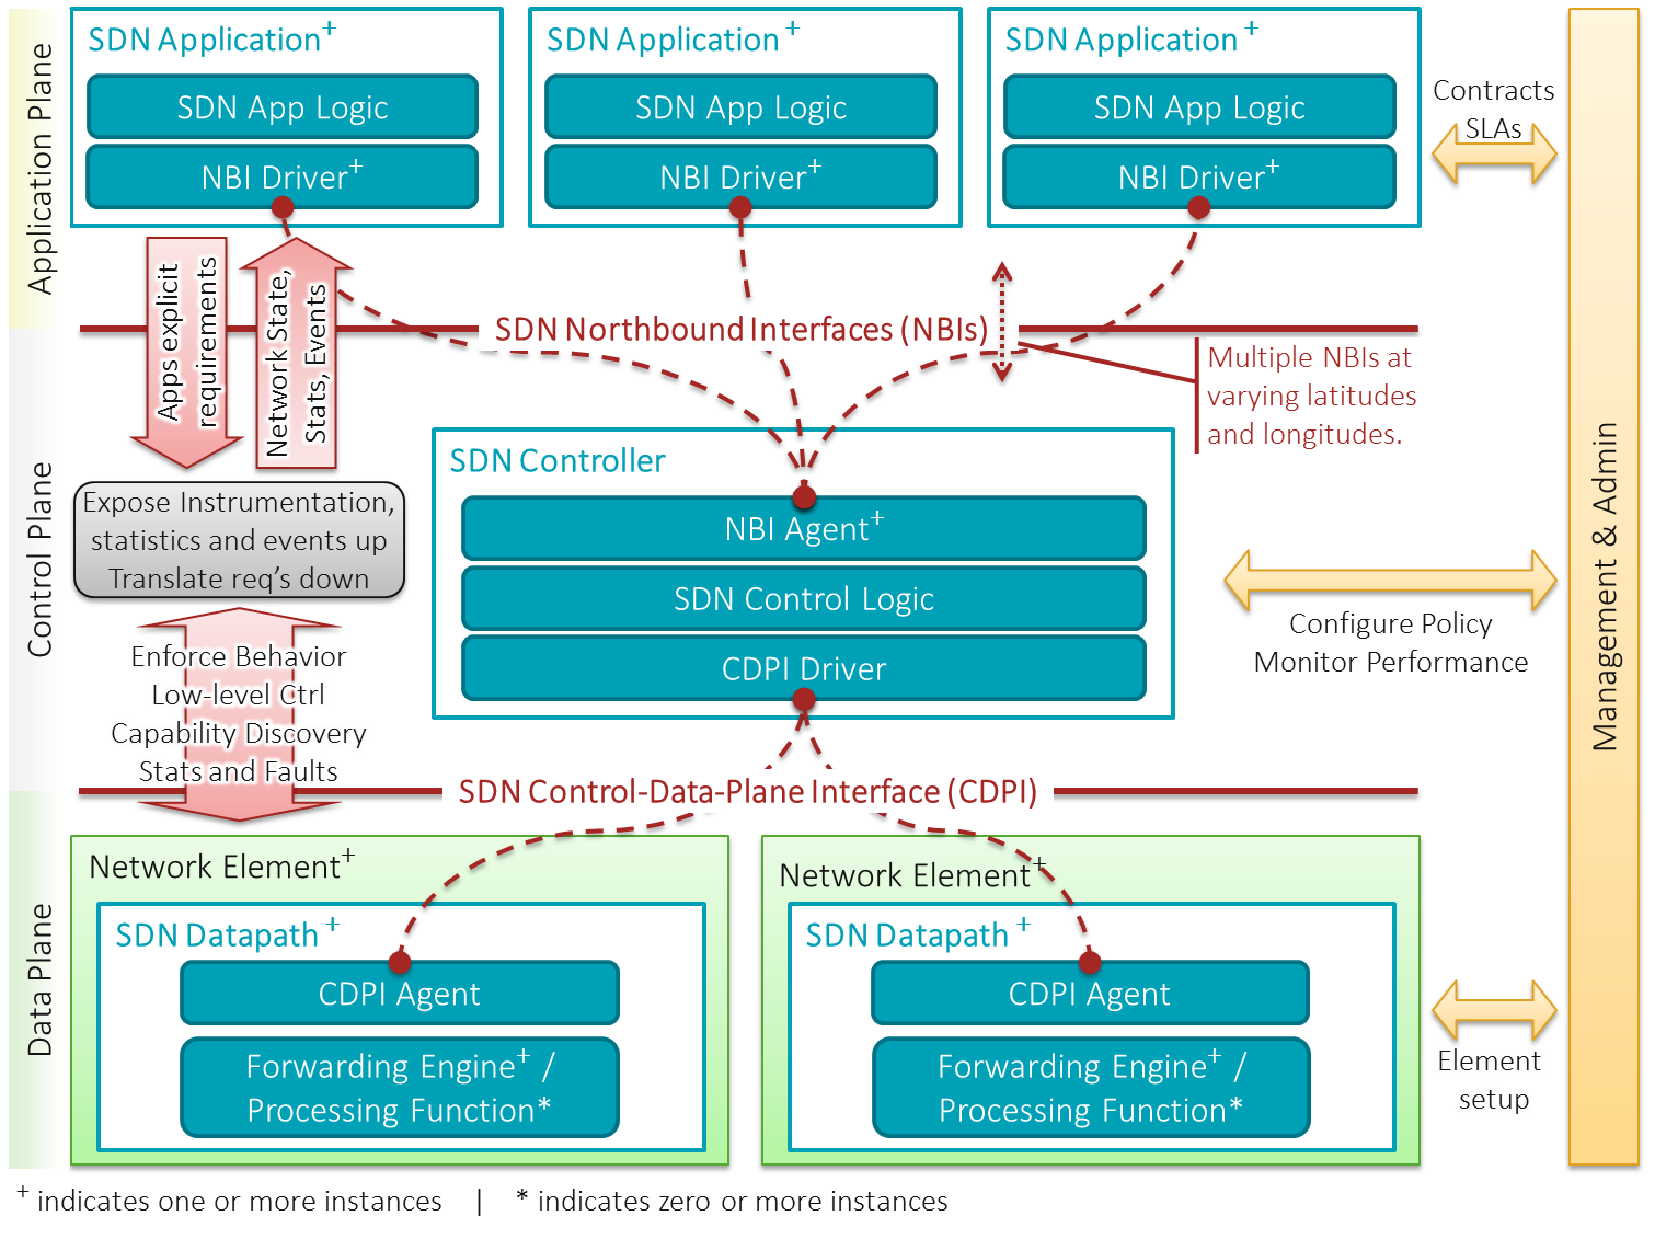
\includegraphics[width=0.6\columnwidth]{SDN-architecture-overview-transparent}
    \caption{High-level SDN architecture Source: \cite{onf_2013:sdn_architecture_overview}}
    \label{fig:sdn_architecture}
\end{figure}

In \cite{onf_2013:sdn_architecture_overview} Open Networking Foundation (ONF) presents a high-level view of SDN architecture along with its major components. Figure 1 depicts a graphical representation of the components and their interactions. At the bottom, The data plane is composed of network elements specialized in treating packages (forwarding), and it communicates with control plane through Control-Data-Plane-Interface (CDPI) also known as Southbound interfaces (SBI). The OpenFlow protocol \cite{mckeown_2008:openflow, kreutz_2015:sdn_comprehensive_survey, onf_2013:sdn_architecture_overview} is the most well-known open standard SBI because its widespread use by vendors and research. At the top, the Applications Plane (AP) implement and orchestrate the business logic and high-level networking functions, such as routing policies and access control. AP communicates their network requirements to the controller plane through the Northbound Interfaces (NBI). In the middle, the SDN controller translates application requirements and exercises low-level control over network elements, providing relevant information to SDN applications. In addition, recent investigations have considered a Management Plane orthogonal to the whole SDN architecture for conducting integrated network management \cite{ESTRADASOLANO_2017:CIM_model}.

\subsubsection{Traffic Engineering}
\label{subsub:background-te}

Traffic Engineering is the process in charge of controlling how traffic flows through the network, using dynamic analysis, prediction and behavior regulation of transmitted data \cite{feamster_2014:road_sdn, awduche_2002:overview_ti, wang_2008:overview_routing_ti, xiao_2000:ti_mpls}. TE uses the methods for measuring and managing network traffic and designs better routing mechanisms to guide and schedule network traffic with aim to optimize the traffic performance and network resource utilization \cite{shu_2016:traffic_measurement_management}. This optimization requires providing appropriate traffic requirements (e.g., throughput, delay, packet loss) while effectively in terms of cost and reliability utilizing network resources (e.g., bandwidth).

TE focuses mainly on four approaches \cite{ian_2014:a_road_map_sdn}: Flow Management, Fault Tolerance, Topology Update, and Traffic Analysis/Characterization. First, maps and controls the traffic flows in the network for optimizing the routing function to steer traffic (from ingress nodes to egress nodes) in the most effective way (\textit{e.g.}, looks for ways to avoid network overhead and provide trade-offs between load balancing and latency). Second refers to ensuring network reliability by providing mechanisms that enhance network integrity and by embracing policies emphasizing network survivability (\textit{e.g.}, seeks to ensure the immediate recovery of the network when a failure occurs in any of its nodes). Third, the Topology Update involves managing the capacity of the network to carry out planned changes (\textit{e.g.}, aims to update the policies of the network in real time and ensure their application in each flow). Last but not least, traffic Analysis/Characterization deals with monitoring the performance of the network and verify the compliance with network performance goals to evaluate and debug the effectiveness of the applied traffic engineering methods (\textit{e.g.}, focuses on mechanisms for monitoring the network, debugging errors, fault detection, data collection, etc.).

Traffic measurement is a prerequisite for traffic management. As part of the Analysis/Characterization approach, traffic measurement is responsible for collecting, monitoring and analyzing real-time network traffic information

%Monitoring is crucial for network management. The management applications require accurate and timely statistics on network resources at different aggregation levels (such as flow, packet and port) [34]. The flow-based programmable networks, such as SDNs, must continuously monitor performance metrics, such as link utilization, in order to quickly adapt forwarding rules in response to changes in workload. . a road map
%falta complementar


\subsubsection{Data Mining}
\label{subsub:background-dm}
Data mining is the knowledge discovery and autonomously extracting useful information from large data stores or sets. The patterns or rules detected by data mining techniques can be used for non-trivial prediction of new information. In non-trivial prediction, information implicitly presented in the data is discovered. DM is an interdisciplinary field that covers areas of statistics, machine learning, data management and databases, pattern recognition, artificial intelligence, and other areas \cite{Dua_2011:DM_ML_Cybersecurity, Dean_2014:BD_DM_ML}. All of these areas relate to particular aspects of data analysis, so they have a lot in common, but each one also has its problems and types of solution.

%\begin{figure}[!ht]
%    \centering
%    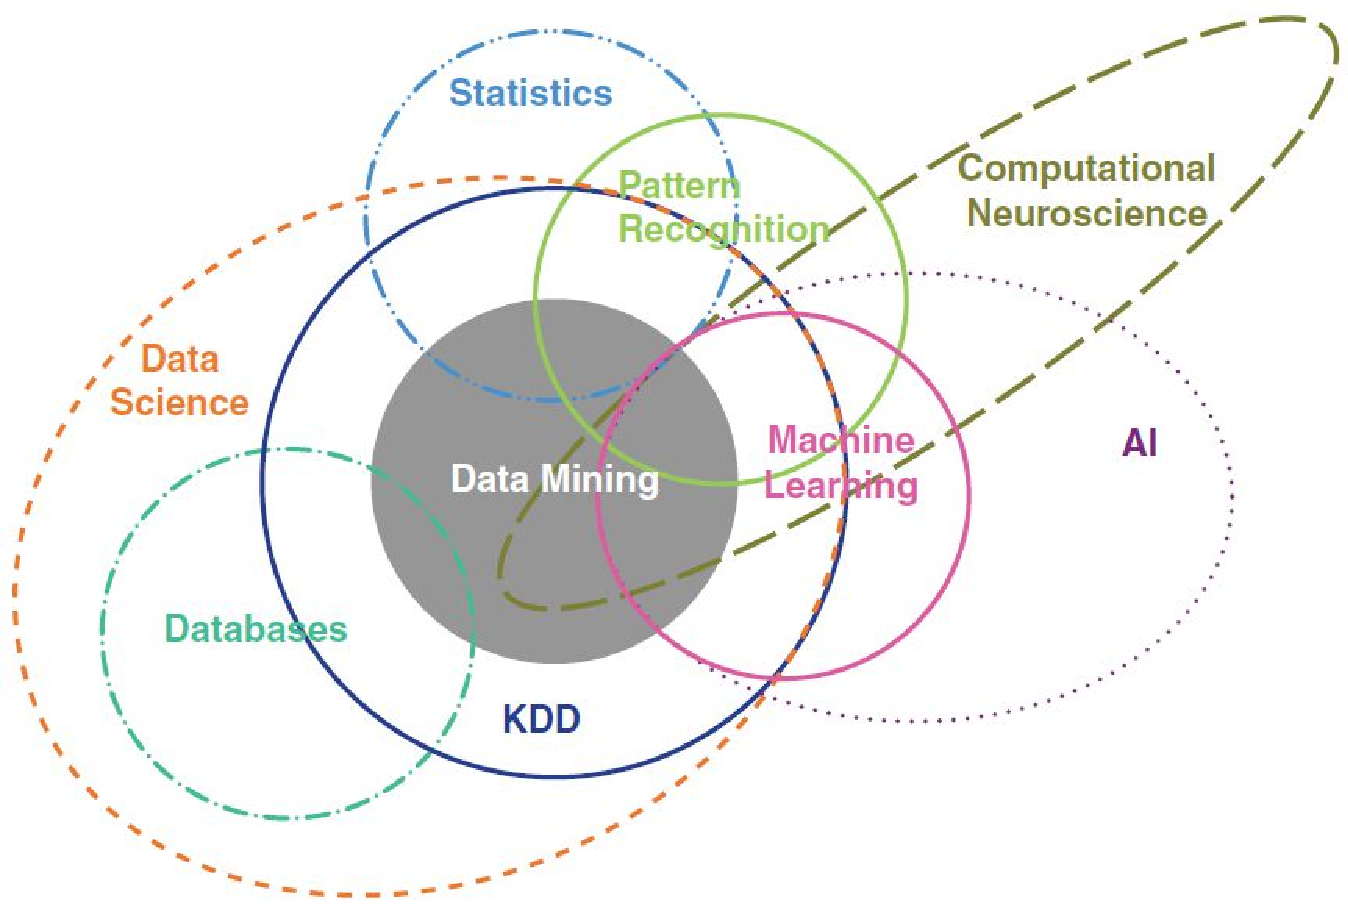
\includegraphics[width=1\columnwidth]{multidisciplinary_dm}
%    \caption{Multidisciplinary Nature of Data Mining. Source: \cite{Dean_2014:BD_DM_ML}}
%    \label{fig:multidisciplinary_dm}
%\end{figure}

Data mining has been used in many domains, including agriculture \cite{efcastillo_2016:agriculture, efcastillo_2015:agriculture, ZHANG_2005:agriculture}, economics \cite{kim_2004:usefulness, nielsen_2004:local}, cybersecurity \cite{Dua_2011:DM_ML_Cybersecurity, Thuraisingham_2003:ciber}, among others. There are two types of data mining methods: supervised and unsupervised. Supervised data mining techniques require a set of examples (instances), commonly known as training data, which are used to define the behavior of the algorithm. The training data consists of a set of attributes and an objective variable (also called class), which is intended to be classified or predicted. Typical examples of supervised mining are classification and prediction. Unsupervised data mining explores the structure of a non-tagged data set (without target variable). This method reveals unexpected characteristics (patterns) and generates new groups (each with different identifiable properties) that obey different patterns. Common examples of unsupervised mining are clustering and mining associative rules.

\subsection{Traffic Engineering for Network Monitoring}
\label{sub:te_in_monitoring}
In the area of IP networks, TE emphasizes the network monitoring under the traditional mechanisms (complex low-level communication protocols, distributed and proprietary network devices) where fine-grained control of traffic monitoring cannot be achieved, and flexibility and extensibility are hard to improve. Recent research efforts have defined solutions to improve this day-to-day approach, while others have harnessed the power of SDN to propose centralized solutions for such control and management, including those that apply Data Mining. In this section, we present some approaches to network monitoring found in the literature.

\subsubsection{Traditional Solutions}
Tcpdump \cite{tcpdump} is a famous tool that allows one to look closer at network packets and make some statistical analysis out of the trace files. Wireshark  \cite{wireshark} adds a user-friendly GUI to Tcpdump and includes many traffic signatures, can be used for accurate, payload-based application identification. Snort  \cite{Roesch_1999:Snort} is a tool for real-time traffic analysis and packet logging, capable of performing content searching/matching and detecting many types of network attacks.  CoralReef \cite{caida}, provides flexible traffic capture, analysis, and report functions. Tstat \cite{Finamore_2010:Tstat} is a passive analysis tool which elaborates tcptrace, and it offers various analysis capabilities with regard to TCP performance metrics, application classification, and VoIP characteristics. 

On the other hand, Cisco NetFlow is a well-known flow monitoring format which uses methods that are installed at network elements as specialized modules. Those modules collect either complete or sampled traffic statistics and send them to a central collector. Another important feature of NetFlow is that its format is not open, and it has been designed only for IPv4 network monitoring \cite{Cisco_2012:netflow}.

SFlow is a proprietary flow sampling method embedded within switches and routers. The sampled information is sent to a central server running software that analyzes and reports on network traffic and provides the ability to continuously monitor application-level traffic flows at wire speed on all interfaces simultaneously \cite{Sflow_2003:sflow}. Sflow, in contrast to the approach used in NetFlow,  the loss of a record does not represent a significant loss of data and doesn't affect the overall accuracy of traffic measurements. 

Another proprietary flow sampling method is JFlow \cite{bandi_2007:JFlow}, which is quite similar to NetFlow. However, these kinds of approaches (store-and-process) present several shortcomings. Firstly, it requires traffic data to be stored and managed for further analysis. This would demand considerable storage space to store the high volume traffic data in a high-speed network environment. Secondly, traffic data are not processed at the time they are produced. So, measurement results cannot be provided in real-time. In addition, these approaches maybe not effective solutions to be applied in SDN systems, such as large-scale data center networks, because of the significantly increased overhead incurred by statistics collection from the whole network at the central controller.

%This may have an impact on time critical network administration tasks, such as abnormal traffic detection and traffic shaping. Therefore, the combination of high-performance traffic collection and real-time data monitoring and analysis is still a challenging target. 

\subsubsection{SDN-based Solutions}

OpenTM \cite{Tootoonchian_2010:opentm} is a query-based monitoring method to estimate the traffic matrix for OpenFlow networks. This method uses built-in features provided in OpenFlow switches to directly and accurately measure the traffic matrix. Subsequently, it uses the routing information learned from the OpenFlow controller to smart choose the switches from which to obtain flow statistics, thus reducing the load on switching elements. It is important to mention that, by measuring network-wide traffic matrix by periodically polling one switch on each flow's, it causes a significant overhead.

FlowSense \cite{Yu_2013:flow_sense}, is a passive push-based monitoring method to analyze control messages between the controller and switches (the network informs the performance changes, rather than query it selves on demand.). It uses the controller messages to monitor and measure network utilization such as the bandwidth consumed by flows traversing the link, without inducing additional overhead. 

In \cite{chowdhury_2014:payless}, authors focus on this trade-off between monitoring accuracy, timeliness, and network overhead. They propose PayLess a monitoring framework for SDN. It provides a flexible RESTful API for flow statistics collection at different aggregation levels. Furthermore, It uses an adaptive statistics collection algorithm that delivers highly accurate information in real-time without incurring significant network overhead. Nevertheless, the monitoring accuracy increases at the cost of increased network overhead.

SWAN \cite{Hong_2013:AHU} utilizes policy rules to allow inter-data center WANs to carry significantly more traffic for higher-priority services while maintaining fairness among similar services. SWAN exploits the global network view enabled by the SDN paradigm to optimize the network sharing policies, which allows WAN to carry more traffic and support flexible network-wide sharing.

In \cite{sgambelluri_2013:of_bsp}, authors modify the OpenFlow architecture to support the protection of segments in networks based on Ethernet. They introduced mechanisms to keep workflows and backups in different priorities, and thus ensure efficient use of network resources when the failed link is recovered.

Kandoo \cite{hassasYeganeh_2012:kandoo} Creates a two-tier hierarchy for controllers: (i) local controllers running local applications as close as possible to the switches, and (ii) a logically centralized controller running globally. A single local controller controls each switch, and each local controller can control multiple switches. The root controller can install flow inputs on the switches of a local controller, delegating the requests in the respective local controller. Kandoo has control channel consumption of order of magnitude lower than normal OpenFlow networks.

BalanceFlow \cite{y_hu_2012:balance_flow} is a controller load balancing architecture for wide-area OF networks, which can partition control traffic load between different controller instances in a more flexible way. All controllers in BalanceFlow maintain their flow-requests information and publish this information periodically through a cross-controller communication system to support load balancing. In BalanceFlow there are two types of controllers, one super controller, and many normal controllers. The super controller is responsible for balancing the load of all controllers, and it detects controller load imbalance when the average number of flow-requests handled by a controller is larger than some threshold of the total flow-requests rate in the network. The threshold is adjustable according to the performance of the super controller, the number of controllers, and the network environment.

\subsubsection{Network Monitoring using Data Mining}
\label{subsub:related_work-te_using_dm}

The authors in \cite{p_wang_2016:traffic_clasification}, propose a QoS-aware traffic classification framework for software-defined networks, which classifies network traffic into different classes according to the QoS requirements, which provide the crucial information to enable the fine-grained and QoS-aware traffic engineering. This technic is located in the network controller so that real-time, adaptive and accurate traffic classification can be realized by exploiting the superior computing capacity, global visibility and inherent programmability of the network controller. Also, uses deep packet inspection (DPI) and semi-supervised machine learning so that accurate traffic classification can be performed.

\cite{poupart_online_2016} presents an online flow size prediction that uses ML techniques (\textit{e.g.}, NN and Bayesian Networks) to identify elephant flows in real datasets. As metrics, they employ True Positive Rate (TPR) and True Negative Rate (TNR), finding that the Gaussian Process Regression is the more robust method. This approach present two problems from the above SDN-based solution. First, it assumes that the data is centralized, however, as observed in FlowSense, collecting data from the switches to a centralized controller increases traffic overhead. In this case the collection of data exponentially increments the traffic overhead because this approach requires per-packet headers; in addition, it would present delay due to data transmission and processing. 

Silva \cite{silva_2015:identification_selection_traffic}, exposes an architecture to identify, extend, and select sets of flow characteristics derived from native OpenFlow counters. This model uses the Selection/Extraction techniques (\textit{e.g.}, Feature Selection, Principal Component Analysis (PCA) and Genetic Algorithm (GA) features to create a set of exceptional flow characteristics to characterize traffic profiles.



%Traffic classification [Li and Moore, 2007]

%Learning algorithms for dynamic resource management in virtual networks [Mijumbi et al., 2014]

%Virtual Network Topology reconfiguration based on BDS for traffic prediction [Morales et al., 2016]
% ----------
% Hypothesis
\section{Hypothesis}
\label{sec:hypothesis}

To address the research question stated in Section \ref{sec:problem_statement}, this thesis proposal raises the following hypothesis: \textbf{The Machine Learning allows intelligent probing on SDN-based networks, improving the accuracy Traffic Monitoring and reducing the corresponding overhead.}
% ----------------------
% Research Contributions
%\section{Research Contributions}
\label{sec:research_contributions}

%\subsection{Gaps}
%\label{subsub:gaps}
%The previous section addressed the research projects related to the control and management of resilience that leverages the power of SDN to propose centralized solutions, including those that apply to data mining. Below are presented the most relevant gaps encountered in related work.

%In this vein, recent research has proposed TE mechanisms that face particular challenges of SDN resilience as discussed in section xxx. From where we have that the techniques of Analysis/Characterization of traffic are closely related to the other approaches TE and with strategies of resilience such as detection of failures and prediction of the congestion of the links \cite{ian_2014:a_road_map_sdn}. In this way, the techniques of Analysis/Characterization become a crucial component in the management of the resilience. However, solutions that analyze the behavior of SDN traffic introduce significant overhead into the network \cite{Yu_2013:flow_sense}. Therefore, proposals such as \cite{chowdhury_2014:payless, Yu_2013:flow_sense, minlan_2013:OpenSketch, Tootoonchian_2010:opentm} seek more efficient Analysis / Characterization mechanisms to achieve high accuracy and low network overhead. Despite the significant advances shown by these proposals, Traffic Analysis/Characterization in SDN continues to be a major research challenge. The challenge that increases if the Analysis/Characterization is done at or near the execution time.

\subsection{Research Contributions}
\label{subsub:research_contributions}
The present thesis proposal aims to achieve the following contributions:

%\begin{itemize}
    %\item A high-level framework that integrates the concepts of ML and SDN into the design of a DCN topology---potentially, switch-centric---for enabling the development of an effective load-balancing solution.
    %\item A mechanism that uses one or a combination of ML techniques for fine-granularity prediction of flow characteristics---potentially, size and time length---in a DCN with the appropriate accuracy and performance requirements.
    %\item A multipath routing mechanism based on SDN that uses the flow characteristics predicted by the ML mechanism for minimizing the maximum load of links---optimizing load-balancing---in a DCN aiming to provide high throughput and low delay while maintaining efficient use of resources.
%\end{itemize}
% ----------
% Objectives
\section{Objectives}
\label{sec:objectives}

\subsection{General Objective}

To introduce a mechanism for Intelligent Probing in SDN by Machine Learning techniques.

\subsection{Specific Objectives}

\begin{itemize}
    \item To design a mechanism based on Machine Learning to intelligent probing in SDN.
    \item To implement a prototype of the proposed mechanism.
    \item To evaluate the prototype in a particular simulated scenario
    %\item To evaluate the proposed model according to its performance, efficiency \footnote{In network management, efficiency is measured concerning traffic statistics and response times. It is also evident that depending on the data mining techniques used will be necessary to use specific metrics; these metrics will be defined in the development of the research.} and effectiveness.
\end{itemize}
% -----------
% Methodology
%\section{Methodology}
\label{sec:methodology}

Figure \ref{fig:methodology} depicts the phases of the scientific research process that will guide the development of this thesis: Problem Statement, Hypothesis Construction, Experimentation, Conclusion, and Publication. Problem Statement, for identifying and establishing the research question. Hypothesis Construction, for formulating the hypothesis and the associated fundamental questions. In addition, this phase aims to define and carry out the conceptual and technological approaches. Experimentation, for testing the hypothesis and analyzing the evaluation results. Conclusion, for outlining conclusions and future works. Note that Hypothesis Construction has feedback from Experimentation and Conclusion. Publication, for submitting and publishing papers for renowned conferences and journals. The writing of the dissertation document also belongs to this last phase.

\begin{figure}[!ht]
    \centering
    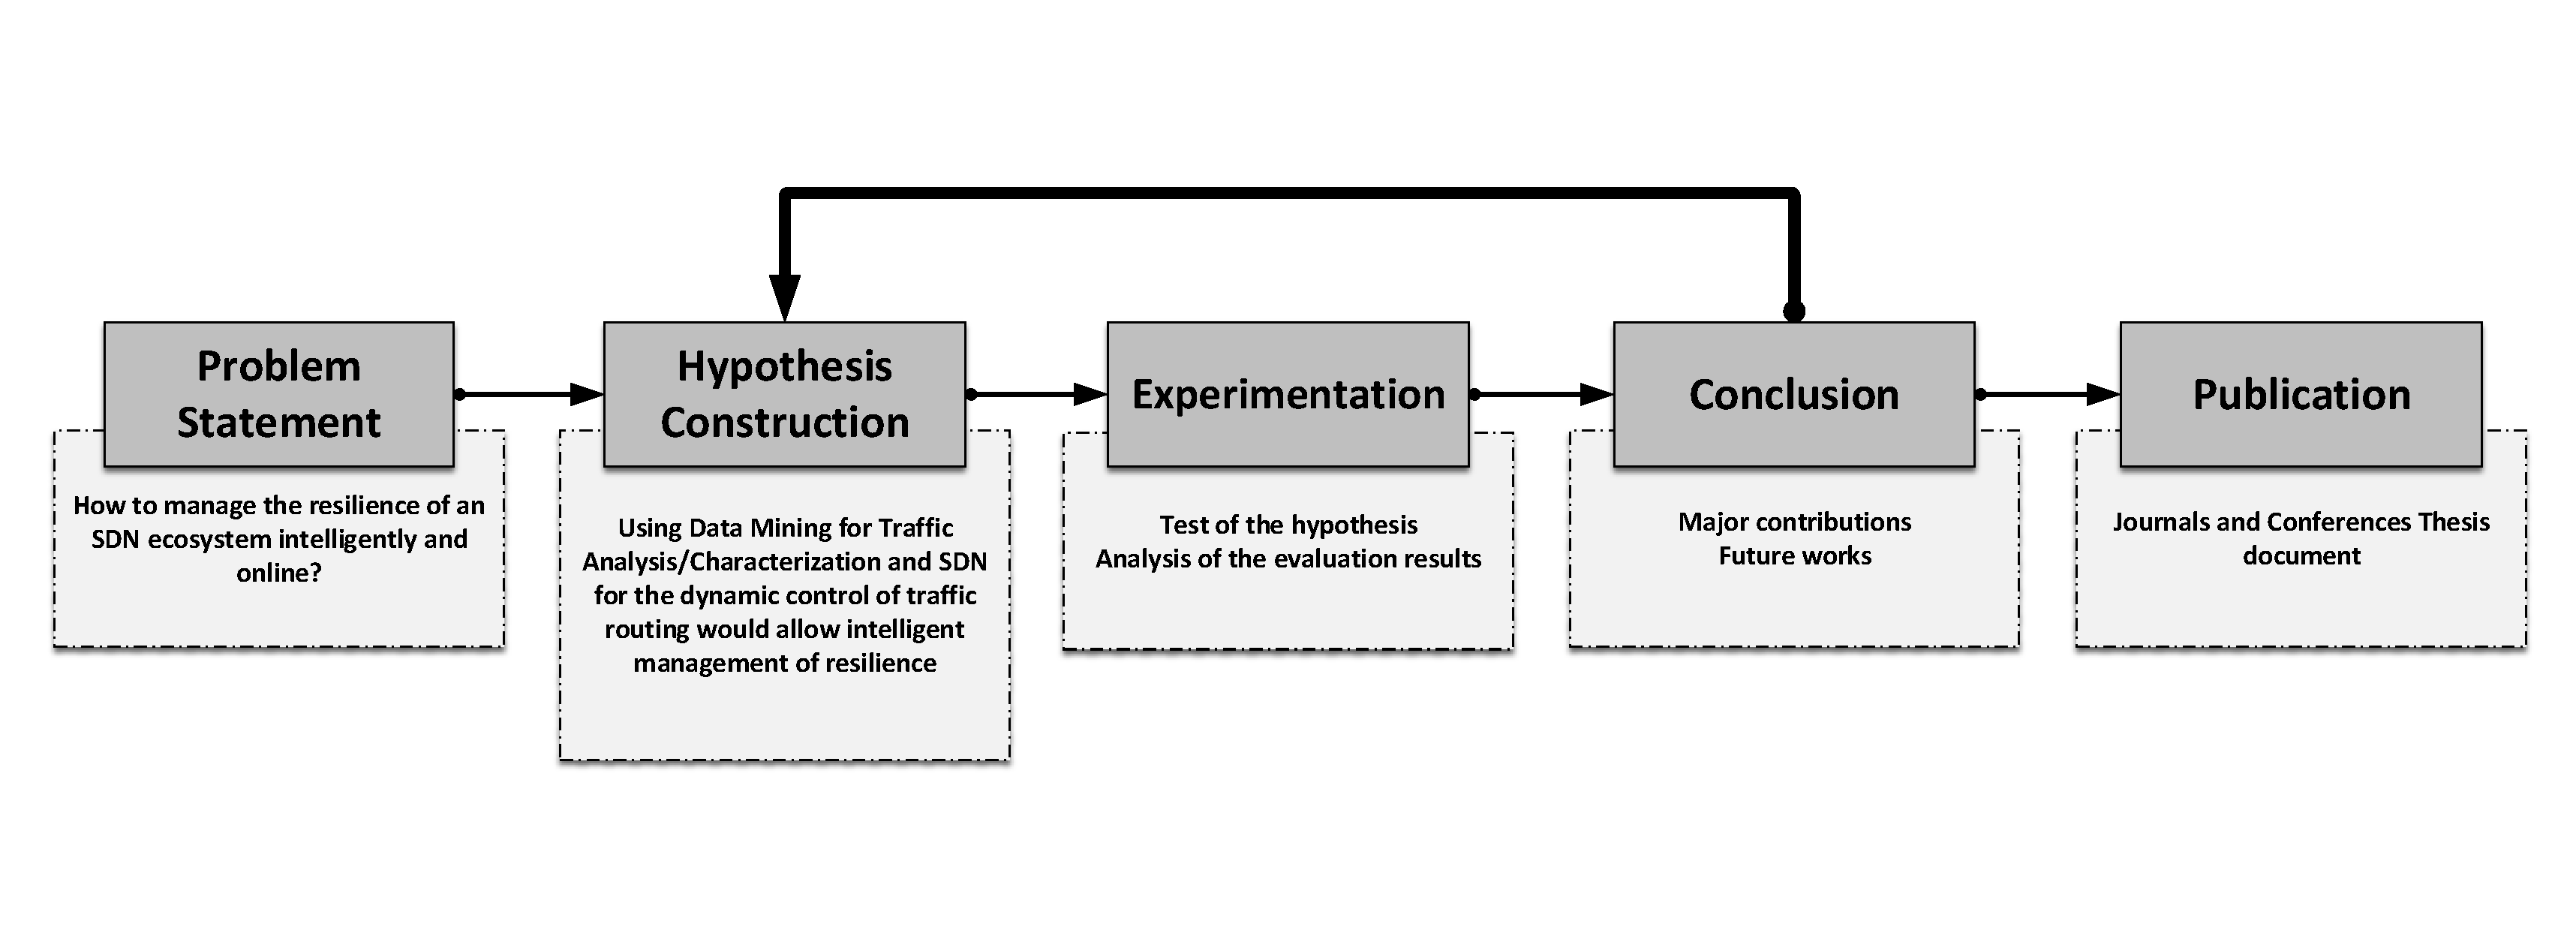
\includegraphics[width=1\columnwidth]{scientific_research_process}
    \caption{Thesis phases}
    \label{fig:scientific_research_process}
\end{figure}
% ------
% Budget
%\section{Budget}
\label{sec:budget}

According to the reference criteria for budget preparation in thesis proposals established by the FIET Research Committee from the University of Cauca and knowing that the value of the point for 2017 is COP\$ 12.939, Table \ref{tab:budget} presents the budget for the proposed thesis project.

\begin{table}[!ht]
    \centering
    \scriptsize
    \begin{tabular}{|l|r|r|r|r|r|}
        
        \hline
        \multirow{2}{0.2\textwidth}{\centering\textbf{Item}} & \multicolumn{4}{|c|}{\textbf{Sources}} &  \multirow{2}{0.15\textwidth}{\centering\textbf{Total}} \\
        \cline{2-5}
        & \multicolumn{1}{|c|}{\textbf{Student}} & \multicolumn{1}{|c|}{\textbf{FIET}} & \multicolumn{1}{|c|}{\textbf{Colciencias}} & \multicolumn{1}{|c|}{\textbf{UWaterloo*}} & \\
        \hline
        
        \hline
        Human resources & 24,842,880.00 & 9,937,152.00 & 72,000,000.00 & 4,456,940.44 & 111,236,972.44 \\
        \hline
        Hardware resources & 1,494,646.15 & 11,981,538.46 & 0.00 & 1,015,384.62 & 14,491,569.23 \\
        \hline
        Software resources & 81,000.00 & 21,000.00 & 0.00 & 60,000.00 & 162,000.00 \\
        \hline
        Library resources & 0.00 & 5,250,000.00 & 0.00 & 12,750,000.00 & 18,000,000.00 \\
        \hline
        Visits and travels & 2,000,000.00 & 4,000,000.00 & 4,000,000.00 & 11,000,000.00 & 21,000,000.00 \\
        \hline
        Publications & 0.00 & 3,000,000.00 & 0.00 & 0.00 & 3,000,000.00 \\
        \hline
        Other resources & 899,413.39 & 2,810,666.85 & 0.00 & 1,049,315.63 & 4,759,395.87 \\
        \hline
        \textit{Subtotal} & \textit{29,317,939.55} & \textit{37,000,357.31} & \textit{76,000,000.00} & \textit{30,331,640.68} & \textit{172,649,937.54} \\
        \hline
        A.U.I. & 0.00 & 25,897,490.63 & 0.00 & 8,632,496.88 & 34,529,987.51 \\
        \hline
        \textbf{Total} & \textbf{29,317,939.55} & \textbf{62,897,847.95} & \textbf{76,000,000.00} & \textbf{38,964,137.56} & \textbf{207,179,925.05} \\
        \hline
        
       % \multicolumn{3}{l}{\tiny{* \textit{Includes the funding from the Government of Canada}}} & \multicolumn{3}{r}{\tiny{\textit{All the values are in COP\$}}}
        
    \end{tabular}
    \caption{Budget of the thesis project}
    \label{tab:budget}
\end{table}

% ----------------
% Submission Terms
%\section{Submission Terms}
\label{sec:submission_terms}

By the end of this thesis project it must be delivered the following items.

\begin{itemize}
    \item A dissertation document that contains the state-of-the-art, the conceptual and technological solutions, and the experimental results.
    \item Additional documents that complement the dissertation document.
    \item A compact disc that gathers all the information generated during the development of this thesis project, including the dissertation document, source code and executable files, related documentation, among others.
    \item Two (1) papers accepted and one (1) submitted in conferences with h-index greater than 20.
    %\item One (1) paper accepted and one (1) submitted in journals from the first quartile (Q1) of the SCImago Journal \& Country Rank (SJR).
\end{itemize}
% ----------
% References
\renewcommand\refname{\vskip -15mm}
\section{References}
\label{references}
\small
\bibliographystyle{ieeetr}
\bibliography{references}
% ------------
\end{document}
